\documentclass{article}% use option titlepage to get the title on a page of its own.
\usepackage{natbib}
\usepackage{geometry}
\usepackage{graphicx}
\geometry{margin=1in}
\title{Introducing an Adolescent Cognitive Maturity Index}
\author{
\parbox{\linewidth}{\centering
Shady El Damaty\,$^{1,2*}$, Valerie L. Darcey\,$^{1,2}$, Goldie A. McQuaid\,$^{2}$, Maria Stoianova\,$^{2}$, Veronica Mucciarone\,$^{2}$, Yewon Chun\,$^{2}$, Marissa L. Laws$^{1}$, Victor Campano\,$^{2}$, Kinney Van Hecke\,$^{2}$, Mary Ryan\,$^{2}$, Emma J. Rose, Diana H. Fishbein\,$^{3,4}$ \& John W. VanMeter\,$^{1}$}
}
\date{\footnotesize{$^{1}$Interdisciplinary Program in Neuroscience, Georgetown University, Washington, District of Columbia, USA
$^{2}$Center for Functional \& Molecular Imaging, Georgetown University Medical Center, Department of Neurology, Washington, District of Columbia, USA
$^{3}$Program for Translational Research on Adversity and Neurodevelopment (P-TRAN), Bennett-Pierce Prevention Research Center, The Pennsylvania State University, University Park, PA 16802
$^{4}$ Translational Neuro-Prevention Research, Frank Porter Graham Child Development Institute, University of Northern Carolina, Chapel Hill, NC} \\  \vspace{5pt} \textbf{Acknowledgments}
Thank you to Melissa Avalos, Amanda Patterson, Maysa Jawdat, Rachel Schroeder, Jaclyn Leiser, Paige Trojanowski, Tomas Clarke, Kelly Martin, Macy Curell, Brittany Eltman, Dana Estefan, and Ileana Pacheco-Colon for running MRI sessions, collecting behavioral data, and coordinating study procedures. }
\begin{document}
\maketitle
%%%%%%%%%%%%%%%%%%%%%%%%%%%%%%%%%%%%%%%%%%%%%%%%%%%%%%%%%%%%%%%%%%
\begin{abstract}
Youth show substantial variation in the rate of physical, cognitive, and social maturation as they traverse adolescence and enter adulthood. Differences in developmental paths are thought to underlie individual differences in life outcomes, however, there remains a lack of consensus on the normative trajectory of cognitive maturation in adolescence. To address this problem, we derive a Cognitive Maturity Index (CMI), to estimate the difference between chronological and cognitive age predicted with latent factor estimates of inhibitory control, risky decision-making and emotional processing measured with standard neuropsychological instruments. Age prediction with latent factor estimates of cognitive skills approximated age within $\pm 10$ months ($r=0.71$). Males in advanced puberty displayed lower cognitive maturity relative to peers of the same age; manifesting as weaker inhibitory control, greater risk taking, desensitization to negative affect, and poor recognition of positive affect.  \\ \\
\textbf{Keywords}: adolescence, cognitive development, age prediction, maturity, dual systems model, maturational imbalance mode
\end{abstract}
%%%%%%%%%%%%%%%%%%%%%%%%%%%%%%%%%%%%%%%%%%%%%%%%%%%%%%%%%%%%%%%%%%
\section*{Introduction}
%%
\paragraph*{Adolescent Cognitive Development}
The transition from adolescence to emerging adulthood is marked by a new cycle of maturation of core cognitive control skills required for adaptive social decision-making in the execution of goal-directed behavior. These skills include active maintenance of goal-related representations in working memory, task switching, inhibitory control of reflexive behavior, weighing of risks versus rewards, and processing emotional context \citep{luna2015}. 
The development of these cognitive skills during adolescence co-occurs with increased sensitivity to reinforcement signals in the form of positive or negative outcomes during social and general task learning \citep{jones2014adolescent, rosenbaum2020valence}. Social signals, such as facial expressions, have been demonstrated to attract automatic attention, modulate hedonia, and serve as reinforcers of socially desired behaviors \citep{teufel2009social,speer2007face}. Strong emotional context during social reinforcement learning captures attention and increases the speed and accuracy of learning new associations \citep{vernetti2017gaze,roper2014value}. Along this vein, several complementary models of adolescent brain development describe adolescence as a period of mismatch between the efficiency of cognitive control and affective salience of reinforcers \citep{CaseyEtAl2008, LunaWright2016}. These models are corroborated by behavioral and neuroimaging evidence suggesting that cognitive skills, and the brain regions that support them, develop together during adolescence.  However, the exact timing of neurocognitive skill maturation and the interaction between cognitive control, risk taking, and emotion processing is not yet fully elucidated \citep{shulman2016dual, duell2016interaction}. The Dual Systems Model claims inhibitory control increases monotonically whereas reward processing is an inverted u-shaped curve that briefly peaks in mid-adolescence and returns to baseline by adulthood. In contrast, the Maturational Imbalance Model proposes inhibitory control and reward processing develop well into adulthood and that greater inhibitory control may temper reward sensitivity by suppressing reflexive responses to hedonic stimuli. Neurophysiological and behavioral evidence supports both models. However, a key distinction to help settle the controversy can be made by tracking the maturation of cognitive skills from adolescence into emerging adulthood \citep{Steinberg2010,somerville2016searching}. The nonlinear characteristics of adolescent cognitive development models have been corroborated with quadratic effects revealed in  risk-taking behavior, risk-taking related neural activity and sex-specific hormone changes over time that extend from ages 9 to 25 \citep{braams2015longitudinal}.
%
\paragraph*{Estimating Cognitive Age}
Although existing models of adolescent cognitive development have been helpful for understanding the transition to adulthood, a key missing aspect is a data-driven operational definition of neurocognitive age or maturity. A more precise definition has the potential to help distinguish sources of variation in development and help translate science for utilitarian social applications by identifying critical developmental windows during which particular interventions may exert the greatest benefits \citep{somerville2016searching}. Early biological models of age based on DNA methylation, transcription and telomere length \citep{baker1988biomarkers, jylhava2017biological}, brain structure \citep{khundrakpam2015prediction,aycheh2018biological,madan2018predicting}, and brain network oxygen metabolism \citep{dosenbach2010prediction, qin2015predicting} have exhibited significant success in predicting age and identifying individual developmental trajectories bench-marked against the average growth curve in the sampled population. However, cognitive age prediction using theory-driven indicator variables obtained from behavioral experiments has yet to be implemented. 
%
% consider the audience - methodologically saavy!
% --> less focus on crystal clear methods
% --> more focus on how it improves models of dev cog neuro
% Limitations of Chronological Age!
% --> Brain Age
%       - let's do this with behavior!!
%
% ---> break main concept of this section down into a few sentences
\paragraph*{Limitations of Model-Free Approach} 
The absence of a complete theoretical model of biological mechanisms underlying age-related changes has been coincident with a proliferation of analytic techniques using large numbers of features to extrapolate sample-specific effects \citep{sagers2020prediction,crimmins2008biomarkers}. Common methods for age prediction typically use big-data-driven approaches, involving the collection of large amounts of data per individual, such as genome-wide RNA transcription, or MRI measurements analyzed using hundreds of thousands of pair-wise correlations between voxels at discrete time intervals. These methods pose an issue in that there are significantly more descriptive features per individual than there are samples in the dataset (i.e., 'the curse of dimensionality'; $p >> n$, \cite{taylor2019}) \textemdash \ a problem that commonly leads to overfitting with standard linear regression. This issue is overcome through the application of data reduction and variable selection techniques, such as principal component analysis or regularized regression, that penalize or eliminate redundant features \citep{lee2017medical}. Model-free techniques have been successful for predicting age within an acceptable error range \citep{cole2017predicting}; however, these models do not always lend themselves to interpretation because variable selection and data reduction can be biased by their cost function, leading to overfitting \citep{babyak2004you}, or confounded by collinear indicators of age, such as motion in fMRI experiments \citep{satterthwaite2013heterogeneous}.
%
\paragraph*{Conceptual Prior for Modeling Maturity} A potential remedy for the curse of dimensionality in age prediction is to build models with data derived from experiments designed to isolate and measure features of age-related change. Currently, there are no applications utilizing behavioral tasks originally developed for testing dual-systems-type models with the goal of estimating cognitive age in typically developing adolescents. Here, we describe a method for computing a cognitive maturity index (CMI) using reaction time, task performance, and other derived metrics from the Continuous Performance (CPT), Wheel of Fortune (WOF), Emotional Face Recognition (EFR), and Temporal Delay Discounting (TD) tasks collected in the Adolescent Development Study \citep{Fishbein2016}. First, confirmatory Factor Analysis (CFA) is used to estimate directly unobservable latent cognitive factors predicted to change with age during adolescence; such as inhibitory control, risk/reward processing, and emotion recognition. The interaction between factors is tested in a structural equation model (SEM) and latent factor estimates of cognitive skills used as predictors in a regularized regression model to predict age. The CMI is defined as the difference between observed and predicted cognitive age for each participant. A high CMI indicates accelerated cognitive maturity relative to the sample mean, whereas a low CMI indicates a relatively lagging developmental trajectory. This work demonstrates that predicting cognitive age using latent constructs is a promising technique that can be scaled with larger neurocognitive datasets to  generate more accurate population estimates for adolescent neurocognitive maturity and further illuminate the interaction between social context and trajectories of neurocognitive development. 
%%%%%%%%%%%%%%%%%%%%%%%%%%%%%%%%%%%%%%%%%%%%%%%%%%%%%%%%%%%%%%%%%%%
\section*{Methods}
%%%%%%%%%%%%%%%%%%%%%%%%%%%%%%%%%%%%%%%%%%%%%%%%%%%%%%%%%%%%%%%%%%%
\subsection*{Participants} 
Early adolescent youth were recruited to participate in the Adolescent Development Study (ADS), a prospective, longitudinal investigation of the neurodevelopmental factors underlying early substance use initiation and the consequences on brain development \citep{Fishbein2016}. Youth ($N=141$) from the Washington, D.C. Metro area were enrolled in 2011 (Table \ref{tab:1}). As of March 2020, participants have completed up to four sequential waves of data collection separated by approximately 18 months. Eligibility at wave 1 included the following criteria: 1) ages 11-13 years, 2) right-handedness, 3) no history of neuropsychiatric disorders or recent head injuries, 4) no self-reported consumption of one or more units of alcohol or other substances and 5) not of direct Asian descent. A total of six participants were excluded following the baseline visit due to: substance use at baseline ($N=2$), autism diagnosis ($N=1$), and high scores on ambidexterity measured with the Edinburgh Handedness Test ($N=3$), \citep{veale2014edinburgh}. Despite attrition, the distribution of sex and race remained approximately the same throughout the study (+/- $0.5\%$). Participants were compensated and reimbursed for travel, when applicable. All youth and caregivers gave their informed assent and consent prior to data collection and study procedures were reviewed and approved by the Georgetown University Institutional Review Board. 
%%%%%%%%%%%%%%%%%%%%%
% Interview
%%%%%%%%%%%%%%%%%%%%%
\subsection*{Interview Procedure and Collected Metrics} Pre-screened, eligible participants were invited for an on-site visit at Georgetown University Medical Center to complete a series of questionnaires and interviews designed to measure neurocognitive developmental traits and capture social and family life. The accompanying primary caregiver was interviewed in a separate room and asked to complete a questionnaire regarding economic status, education, and the difficulty of acquiring basic needs such as food, healthcare, and housing \citep{bornstein2003socioeconomic}. Socioeconomic Status (SES) was estimated from these responses by converting the family’s household income to z-scores, averaging both guardian/parents' years of education, converting the average to a z-score, and lastly averaging the income and education z-scores for the final SES measure \citep{manuck2010ses}.
%%%%%%%%%%%%%%%%%%%%%
% Anthropometrics
%%%%%%%%%%%%%%%%%%%%%
\paragraph*{Anthropometrics} Adolescents had their height and weight measured and completed the Pubertal Development Scale \citep{carskadon1993self} to measure body-mass index (BMI) and physical changes with age at each wave. Pubertal development scores were derived from from reported changes in height, body hair, complexion, vocal pitch, breast size, and menarche. Respondents responded with: “has not yet begun,” “has barely begun,” “is definitely underway,” or “is complete” for each puberty related physical features queried by the instrument. 
%%%%%%%%%%%%%%%%%%%%%
% Instruments
%%%%%%%%%%%%%%%%%%%%%
\paragraph*{Instruments} All participants were assessed for verbal and performance IQ using the Kaufman Brief Intelligence Test (KBIT), \citep{kaufman2004kaufman} and  completed The Behavioral Inhibition System/Behavioral Activation System (BIS/BAS) Scale  to provide a measure of appetitive and avoidant behavioral tendencies \citep{carver1994behavioral}. The BAS is divided into three subscales measuring funseeking (BAS-FS; four items, ex. "I will often do things for no other reason than that they might be fun."), independent drive (BAS-D; four items, ex. "I go out of my way to get things I want") and reward responsivity (BAS-RR; five items, ex. "When I get something I want, I feel excited and energized") used to measure self-reported idiosyncratic differences in temperament and personality underlying reinforcement sensitivity \citep{corr2004reinforcementsensitivity}. Participants were asked on a four-point scale how well a particular statement characterized them (1:strongly agree to 4:strongly disagree).
%%%%%%%%%%%%%%%%%%%%%
% Neurocognitive Tasks
%%%%%%%%%%%%%%%%%%%%%
\subsection*{Neurocognitive Tasks}  Participants completed the Continuous Performance and Wheel of Fortune tasks while undergoing functional MRI (Siemens Tim Trio 3T Scanner) during waves one through three. Stimuli were projected onto a screen and reflected into the participant's field of view using a mirror. Participants responded using fiber optical button boxes. The Emotional Face Recognition and Temporal Discounting tasks were completed outside of the scanner on a laptop in a private behavioral testing room in the first three waves. The Facial Emotion Recognition Task was administered with E-Prime 1.2. All other neurocognitive tasks were built and presented with the E-prime Stimulus Presentation Software Version 2.0 \citep{schneider2002prime}. 
%%%%%%%%%%%%%%%%%%%%%
% CPT
%%%%%%%%%%%%%%%%%%%%%
\paragraph*{Continuous Performance Task (CPT)} The continuous performance task was used to measure impulsivity and inhibitory control of reflexive actions \citep{horn2003response}.  Participants viewed five blocks of $30$ letters presented one-at-a-time for a $200$ms duration (150 total trials). Each block was separated by a "cool-down" period in which a gray fixation cross was presented for $1300$ms. Participants were instructed to press the right-hand button box as quickly as possible for all letters except “Q”. The lure "Q" appeared 27 times in the task. The sequence of letters was the same across all participants.  Signal Detection Theory metrics were utilized for analyzing CPT behavior \cite{stanislaw1999calculation}. 'Hits' were defined as correct button presses to target letters and 'Misses' as failure to respond to a target letter. 'False-Alarms' were defined as an incorrect response to the the lure "Q", whereas 'Correct Rejections' were defined as correct inhibition of response. Discriminative sensitivity to lures was measured by the $d'$ variable, $d'=\phi^{-1}( Hits ) - \phi^{-1}( False Alarms )$, and response-bias calculated by utilizing the natural log-transformed beta estimate, $ \beta = 0.5*\Big[\phi^{-1}(FalseAlarms)^{2} - \phi^{-1}(Hits)^{2}\Big]$; where $\phi^{-1}$ is the inverse probability distribution function  \citep{forbes2011statistical}. 
%%%%%%%%%%%%%%%%%%%%%
% WOF
%%%%%%%%%%%%%%%%%%%%%
\paragraph*{Wheel of Fortune Task (WOF)} A modified version of the Wheel of Fortune (WOF) task was administered to test propensity of risk-taking and gambling strategies \citep{ernst2004wheeloffortune}. The task was divided into three runs of 30 trials. In each trial, a "wheel" appeared on the screen that portrayed the probabilities of winning different amounts of virtual money. Participants were instructed to select between large monetary gains with a low probability (high-risk) or small monetary gains with high probability (low-risk) and indicated their choice using button boxes placed in their left and right hands (corresponding to choice of the left and right sides of the wheel, respectively). Winning probability varied pseudo-randomly between a $10:90\%$ split (occurring $32$ to $42$ times of a total $90$ trials) and a $30:70\%$ split (occurring $48$ to $58$ times). The quantities of money assigned to the left and right side of the wheel varied between a \$$1$ - \$$9$ for the low risk choice or a \$$2$ - \$$18$ split for the high risk choice, when the wheel was split $10:90$. The quantities similarly varied between \$$3$ - \$$7$ or a \$$9$ - \$$21$ split when the wheel was divided $30:70$.  These values and proportional assignments assured that the expected value (EV) appeared equal for a winning selection independent of risk (e.g., $30\%$ chance of winning \$$7 = $\$$2.10$ EV vs. $70\%$ chance of winning \$$3 =$ \$$2.10$ EV).  Spatial position of the rewards varied evenly, with the larger reward appearing on each side $50\%$ of the time.  The wheel was visible until the participant made their selection, or for a maximum of $3000$ms, followed by a $3000$ms delay after which feedback was presented indicating whether the participant had won or lost the selected dollar amount, along with their cumulative winnings up to and including that trial.  Participants automatically lost the higher dollar amount if no decision was made before $3000$ms had elapsed.  Each run began with a $6000$ms fixation, and the inter-trial interval was varied based on a Poisson distribution between $2500$ to $10000$ms. The total quantity of money won or lost would be reset to \$$0$ at the beginning of each run. Participants were encouraged to improve upon the amount they won in the next run.  Participants were encouraged to respond as if their gains and losses were real, however no real money or physical reward was given. Task performance was analyzed using the probability of high vs. low risk decisions, the reaction time to make those decisions and the cumulative winnings at each run. Anticipatory responses were defined as trials $<200$ms reaction time and discarded from analysis as outliers.
%%%%%%%%%%%%%%%%%%%%%
% EFR
%%%%%%%%%%%%%%%%%%%%%
\paragraph*{Emotional Face Recognition Task (EFR)} Participants viewed $70$ photographs (grayscale images, $284$ x $351$ pixels, resolution = $96$ dpi) from the NimStim dataset, which includes images of twenty-nine professional actors aged $21$-$30$ years ($12$ female, $17$ male, $14$ European-American, $10$ African-American, $3$ Asian-American $2$ Latino-American) instructed to pose for expressions of seven emotions: happiness, surprise, sadness, anger, disgust, fear and neutral \citep{tottenham2009nimstim}. To prepare for the task, participants were presented showcards with labels of each of seven emotions and asked to describe each of the emotions followed by a practice trial for each emotion. For each trial, a photograph appeared for a maximum duration of $5000$ms along with seven labels for each of the emotions. Participants were instructed to click on the emotion with a mouse to advance to the next trial. The image disappeared after $5000$ms and labels remained until a response was made. Trials were separated by an inter-trial interval of $3000$ms, during which time participants viewed a white screen. No actor was shown with the same emotion more than once. The accuracy and reaction time for disgust, anger, sadness and fear were averaged together to compose estimates of performance for recognizing negative emotion. Positive emotion recognition performance was derived from reaction time and accuracy for happy faces only. 
%%%%%%%%%%%%%%%%%%%%%
% TD
%%%%%%%%%%%%%%%%%%%%%
\paragraph*{Temporal Delay Discounting Task (TD)} Individual preference between small, immediate vs. large, delayed rewards was tested by offering participants a forced choice between two options: "Would you rather have \$$X$ now or \$$X+Y$ in $Z$ days?" The delay of rewards, $Z$, was varied from zero, one, two, ten days, 1 month, half a year and one year. The immediately available amount, $X$, was determined using a random adjustment procedure that updated the current choice based on previous choices. Immediate reward amounts varied from \$$0.50$ to \$$10$ while the delayed reward value $X+Y$ was fixed at \$$10$. The propensity for discounting the objective value due to delayed receipt was computed as the area under the curve (AUC) using the trapezoidal method: $AUC = \sum_{t=0}^{t=k} (d_{t+1}-d_t)*(v_t+v_{t+1} /2)$, where $t$ is the current normalized delay point, $k$ the maximum delay and $v$ the indifference value at that point \citep{Borges2016,olson2007adolescents, myerson2001area}. Indifference points reflecting the subjective value of the immediately available reward at a given delay were normalized to the maximum award value of \$$10$ and plotted across annualized time delays. As described above, trapezoids formed by normalized subjective values at each normalized delay contributed to AUC in the range from $0-1$.  A large AUC indicates participants are more likely to prefer large but delayed rewards whereas a lower AUC indicates preference for immediate gratification. In order to elicit behavior reflective of the participant's actual preferences, participants were informed that they would receive either a \$$5$ or \$$10$ reward based randomly on their choices in the task prior to the task. 
%%%%%%%%%%%%%%%%%%%%%
% Analysis Methods
%%%%%%%%%%%%%%%%%%%%%
\vspace{2pt}
%%%%%%%%%%%%%%%%%%%%%%%%%%%%%%%%%%%%%%%%%%%%%%%%%%%%%%%%%%%%%%%%%%%%%%%
\subsection*{Statistical Analysis} Data were converted from double-entered paper records, Qualtrics survey exports, and E-prime task outputs then consolidated into a single long-format data frame containing an observation for each participant at each wave. Next, descriptive statistics and assessments of multivariate normality were performed with the Arsenal (3.5.0), MVN (5.8, \cite{MVN}) and DescTools (0.99.36, \cite{DescTools}) packages in R version Orange Blossom (1.2.5033, \cite{R}). Participants with high DUSI-R Lie scores (N=23; Lie$>6$) were excluded from analysis \citep{dalla2003effects}. Demographics for the excluded participants did not significantly differ from the retained group. Scored neurocognitive and sociodemographic measures were correlated with age to identify and confirm expected bivarate relationships with development, including that of age-related changes in neurocognitive skills as revealed by EFR, CPT, WoF, TD task performance. Longitudinal effects of task performance by age were performed using the lmer R package to account for hierarchies of repeated measures in multi-level models \citep{lmer}. Task performance at each wave of data collection was modelled as a nested factor within participants and used to estimate the average intercept and rate of change across all participants and within subgroups controlling for random effects attributable to individual differences. First, we assessed the Confirmatory Factor Analysis (CFA) was implemented with the Lavaan R package (0.6-6) to estimate latent factors for inhibitory control (CPT), risk/reward processing (WOF/TD), and emotional face recognition (EFR) \citep{Lavaan}. Latent factor analysis is a statistical method for estimating an underlying mechanism that can only be indirectly measured through indicators derived from experimental constructs \citep{finch2015latent}. Latent factor estimates are obtained by averaging the unique contribution of each indicator variable after controlling for the shared variance across indicators to satisfy the local independence principle \citep{sobel1997measurement}. The resulting estimate is considered as a weighted combination of the residual covariance between indicator variables used to approximate the inferred latent factor, where the correlation between two indicator variables is permitted when they are both caused by the underlying latent variable \citep{cooper2019neuroimaging}. This approach serves to reduce the number of variables required to model a hypothesized cognitive phenomenon and helps minimize the contribution of residual error on tests of statistical inference; both useful and necessary requirements for building predictive regression models that avoid over-fitting with collinear predictors. Maximum likelihood estimation with full information maximum likelihood (FIML) was used to adjust CFA parameter estimates for missing data \citep{cham2017full}. The latent factors were standardized to allow for free estimation of factor loadings and post hoc testing \citep{HuTzeBentler1998}. The model fit of the implied structural relationships was assessed with $\chi^2$ Goodness of Fit referenced against a null model with $0$ factor loadings, the Root Mean Square Error of Approximation (RMSEA), the Comparative Fit Index (CFI) and the Tucker-Lewis Index (TLI; \cite{KennyEtAl2015,HuTzeBentler1999, wu2009evaluating}). Path and structural models were visualized with the semPlot R package (1.1.2). The standardized latent factor estimates of inhibitory control, risk taking and facial emotion recognition were used to predict age with regularized linear regression models implemented in the glmnet R package (4.0-2) using leave-one-out cross-validation for estimation of model hyperparameters and a 50\% random split across participants between training and test datasets \citep{FriedmanHastieTibshirani2010, friedman2009glmnet}. Cross-validated model performance was estimated by computing the $R^2$ from the mean cross-validated error divided by the variance of observed age in the test sample across the regularization rate ($\lambda$) and penalty factor ($\alpha$; $0 = $Ridge Regression, $0.5 = $ Elastic Net, $1 =$ Least Absolute Shrinkage and Selection Operator) hyper-parameter estimates. The minimum $\lambda$ at the highest $R^2$ was used to calculate regression coefficients in the training sample. The cognitive maturity index was estimated as the difference in the observed and predicted age for each participant. 
%%%%%%%%%%%%%%%%%%%%%%%%%%%%%%%%%%%%%%%%%%%%%%%%%%%%%%%%%%%%%%%%%%%%%%%%%%%
\section*{Results} 
%%%%%%%%%%%%%%%%%%%%%%%%%%%%%%%%%%%%%%%%%%%%%%%%%%%%%%%%%%%%%%%%%%%%%%%%%%%%%%%%%%%%
% Latent Factor Analysis
\subsection*{Latent Factor Analysis of Cognitive Metrics} 
%%%%%%%%%%%%%%%%%%%%%
% Inhibitory Control
%%%%%%%%%%%%%%%%%%%%%
\paragraph*{Inhibitory Control} 
The inhibitory control latent factor (ICLF) was characterized by consistently careful responses and greater target discrimination in the CPT, along with overall behavioral caution measured by the BIS. The ICLF  was estimated using the CPT response time standard deviation, log transformed response bias, $ln(\beta$), target discrimination, $d'$, and the BIS part of the BIS/BAS. Response time standard deviation was selected for the model \textit{a priori} because mean reaction time did not significantly vary trial-by-trial across participants except at the beginning of a block (Figure S1). Additionally, participants were instructed to press the response button as fast as possible and variations in responses were typically only observed circa false alarm trials during which more cautious participants would modify their pace to avoid errors. Task performance improved from wave one to three independent of task learning effects (Figure S2, S3). The fitted relations were significant compared to a null model with 0 factor loadings between all measures, residual covariances, and the latent variable estimate (Table \ref{tab:2}; $CLI = 1.0$; $TLI = 1.018$; $RMSEA < 0.01$, $p = 0.91$). Greater discriminative ability between false alarms and targets was significantly inversely correlated to response bias ($-0.46\pm0.14$; $Z=3.36$; $p=0.001$) and was associated with greater variation in response time to targets ($0.30\pm0.09$; $Z=3.36$; $p=0.001$), suggesting participants modified their behavior and responded with more consistent timing as they learned the task (Figure \ref{fig:1}). This was corroborated by a strong linear relationship between $d'$ and the average response time to targets (Figure S4; $0.57\pm0.05$; $Z=12.11$, $p<0.001$). Response time variance to targets interacted inversely with false alarm response time to predict $d'$ ($-0.08\pm0.02$;  $Z=-3.35$, $p < 0.001$) indicating that rapid response to early false alarms led to greater caution later in the task, resulting in overall improvement in target/lure discrimination and CPT performance. Response time variation was uncorrelated between target and false alarm trials ($0.07\pm0.09$; $Z=0.70$, $p=0.48$) demonstrating that each provided a statistically independent contribution to ICLF. The significant contribution of the BIS to estimation of ICLF revealed that inhibitory control in the CPT was also indicative of generic internalizing behavior and disposition towards caution. The ICLF did not vary by sex, or BMI, but was found to significantly increase with SES ($0.267\pm0.053$; $Z=4.99$, $p<0.001$) and pubertal development ($0.14\pm0.06$; $Z=2.22$, $p=0.03$). 
%%%%%%%%%%%%%%%%%%%%%
% Risk/Reward
%%%%%%%%%%%%%%%%%%%%%
\paragraph*{Risk Taking} The risk/reward evaluation latent factor (RRLF) was found to drive impulsive risk taking and a preference for immediate rewards. The RRLF was estimated using probability of high risk decisions, cumulative winnings and response time in the WOF task, and area under the curve of TD performance. Overall, RRLF was characterized by greater risky decisions, moderate response time for high risk options, longer response time for low risk decisions, significantly poorer cumulative winnings and stronger propensity for immediate rewards in the TD task (Table \ref{tab:3}). The model fit to the data significantly improved by allowing free estimation of covariance between the probability of making a high risk decision and response time, and between low and high risk response times. The fitted relations with these free parameters revealed a significant fit of the covariance structure compared to a null model with 0 factor loadings between all measures, residual covariances, and the RRLF estimate ($CLI = 1.0$; $TLI = 1.0$; $RMSEA = 0.005$, $p = 0.846$). The estimate of the covariance between response time and the probability of making a high high risk decision revealed that risky decisions occurred more quickly than carefully evaluated low risk options ($-0.121\pm0.031$; $Z=-3.849$, $p<0.001$). Overall, the RRLF was related to greater risk taking in the WOF task, which resulted in poor cumulative winnings due to high probability of loss and consequently running a negative balance. RRLF did not significantly covary with sex, PDS, BMI, or SES.
%%%%%%%%%%%%%%%%%%%%%
% Emotion
%%%%%%%%%%%%%%%%%%%%%
\paragraph*{Emotional Face Recognition} Performance in the EFR task was used to derive latent factors of positive and negative emotional face recognition (EPLF/ENLF). Latent factors were estimated using the mean and standard deviation of response time and accuracy to recognize angry, fearful, sad, or disgusted (negative) and happy (positive) facial expressions. The model fit was improved significantly by permitting free covariation between mean reaction time to negative and positive faces, negative and positive emotion recognition accuracy, and between standard deviation and mean response time for both negative and positive emotions. The proposed model structure explained a significant proportion of the covariance between task metrics and provided an excellent fit compared to a null model (Table \ref{tab:4}; $CLI = 0.978$; $TLI = 0.942$; $RMSEA = 0.073$, $p = 0.115$). Perceptual processing of positive emotional faces often resulted in correct emotion recognition, but was associated with generally longer and more variant time to recognition, reflecting difficulty in distinguishing between happy and other facial expressions. Perceptual processing of negative emotional faces often resulted in correct recognition with quick and consistently low variation in recognition time. The structural equation model revealed perceptual processing performance for negative emotions was inversely related to positive emotion processing (standardized estimate $-3.44\pm1.85$; $Z=-1.86$, $p = 0.063$). This result suggests participants generally tuned to facial expressions of negative affect were more likely to exhibit rapid and inaccurate recognition of positive affect. ENLF, but not EPLF, was found to increase with SES ($0.16\pm0.07$; $Z=2.11$, $p = 0.036$) and BMI ($0.04\pm0.02$; $Z=2.65$, $p=0.008$), suggesting youth from prosperous, more educated, households are more sensitive to recognizing facial expressions of negative affect but do not possess comparable performance on positive affect recognition. No significant relationship between ENLF and sex or PDS was revealed. Greater physical maturation measured with PDS was related to lower EPLF scores ($-0.70\pm0.15$; $Z=-4.55$, $p<0.001$), indicating that physically mature youth exhibit faster, less variable, recognition time and poorer accuracy for happy facial expressions. No relationship between EPLF and SES, BMI, or sex was found.
%%%%%%%%%%%%%%%%%%%%%%%%%%%%%%%%%%%%%%%%%%%%%%%%%%%%%%%%%%%%%%%
% Interaction SEM
%%%%%%%%%%%%%%%%%%%%%%%%%%%%%%%%%%%%%%%%%%%%%%%%%%%%%%%%%%%%%%%
\subsection*{Structural Equation Model of Cognitive Factors} A structural equation model was constructed to explore the interaction between the identified latent factors and their indicator variables (Figure \ref{fig:2}). Significant covariations were identified between the constituent cognitive latent factors compared to a null model ($CLI = 0.95$; $TLI = 0.93$; $RMSEA = 0.047$, $p = 0.64$). ICLF was found to significantly reduce RRLF, suggesting greater inhibitory control can curtail a propensity for risk taking ($-0.22\pm0.10$; $Z=-2.16$, $p<0.031$). Greater inhibitory control also predicted greater sensitivity to negative emotional faces ($0.55\pm0.26$; $Z=2.09$, $p = 0.037$) and effected faster recognition time for all emotions at the expense of recognizing happy facial expressions. As previously noted, elevated ENLF was inversely correlated with EPLF. No relationship was found between RRLF and negative or positive emotional processing.
%%%%%%%%%%%%%%%%%%%%%%%%%%%%%%%%%%%%%%%%%%%%%%%%%%%%%%%%%%%%%%%
% Neurocognitive Maturity Index
%%%%%%%%%%%%%%%%%%%%%%%%%%%%%%%%%%%%%%%%%%%%%%%%%%%%%%%%%%%%%%%
\subsection*{Cognitive Maturity Index} Linear ordinary least squares regression was used to test ICLF, RRLF, EPLF, and ENLF as predictors of chronological age to explore the utility of building a predictive model of neurocognitive age. Inhibitory control ($0.72\pm0.01$; $Z=7.50$, $p<0.001$) and negative affect perceptual processing ($0.35\pm0.14$; $Z=2.44$, $p=0.015$) significantly increased in efficiency with age, whereas risky reward taking ($-0.22\pm0.10$; $Z=-2.35$, $p = 0.019$) and positive affect recognition ($-0.16\pm0.10$; $Z=-1.52$, $p=0.129$) declined. Ridge regression ($\alpha = 0$, $\lambda = 0.083$) with latent factors predicted age in a split-half test sample within a mean absolute error of $\pm 10.11$ months ($R^2=0.51$; Figure \ref{fig:3}), significantly more accurately than by training on the original indicator variables used to generate the latent variable estimates ($R^2=0.16$). The difference between predicted and observed age, defined as the cognitive maturity index (CMI), was computed for each participant. A lower CMI value indicated delayed maturity and a higher value indicated accelerated maturity of cognitive skills, relative to the average development of in-sample youth at a given age. Greater CMI correlated with lower BMI (Pearson's $R=-0.24$, $p<0.001$), slower pubertal development ($R=-0.20$, $p<0.001$), lower BAS-D ($R=-0.16$, $p<0.001$), higher IQ scores ($R=0.20$, $p<0.001$), and lower DUSI-R problem scale scores on: substance use ($R=-0.20$, $p<0.001$), health risk ($R=-0.16$, $p<0.001$), and, lastly, risk for violence ($R=-0.28$, $p<0.001$). No significant relationship was found between SES and CMI, or between any of the other BIS/BAS scales and CMI. Advanced pubertal development ($-0.67\pm0.089$; $Z=-7.47$, $p<0.001$) interacted with sex ($-2.44\pm0.39$; $Z=-6.21$, $p<0.001$) to predict greater CMI in more fully developed females compared to males (interaction effect estimate $0.82\pm0.16$; $Z=5.30$, $p<0.001$).
%
%%%%%%%%%%%%%%%%%%%%%%%%%%%%%%%%%%%%%%%%%%%%%%%%%%%%%%%%%%%%%%%
% DISCUSSION
%%%%%%%%%%%%%%%%%%%%%%%%%%%%%%%%%%%%%%%%%%%%%%%%%%%%%%%%%%%%%%%
\section*{Discussion} The distinction between chronological and biological age has been explored in great detail but not yet extended to account for different trajectories of neurocognitive maturation during adolescence. The current study shows development of a novel method for identifying behavioral hallmarks of cognitive development that can be used to estimate population-relative maturity in adolescents and has significant implications for predicting adverse life outcomes in emerging adulthood. Theory-driven variable reduction was implemented with regularized regression for optimized age-prediction accuracy ($\pm 10$ months) than has been previously possible with neuroimaging datasets ($\pm1$ year), which typically incorporate a massive number of features, leading to overfitting \citep{cole2017predicting, franke2012brain}. 
\vspace{4pt}
%%%% Latent Cognitive Factors
\paragraph*{Adolescent Cognitive Development} Models of adolescent neurocognitive development have reached a general consensus that risk taking and cognitive control change significantly during adolescence \citep{Steinberg2010}. However, agreement on the dynamics and timing of this transition has remained elusive. The Dual Systems Model describes the approach to maturity as a linear age-related increase in cognitive control that catches up over time with the inverted u-shaped development of the reward system \citep{Steinberg2005}. Elevated risk-taking and reward sensitivity are considered to be transient events in the transition to adulthood before returning to a pre-adolescent baseline. In contrast, the Maturational Imbalance Model suggests both the reward and cognitive control systems develop exponentially over time, though at different rates, and reach a stable plateau that continues into adulthood \citep{CaseyEtAl2008}. The early emergence of elevated risk/reward processing is considered to be tempered by later maturation of cognitive control in the Maturational Imbalance Model \citep{somerville2010developmental}. Further elaborations of these models have included an additional emotional processing component that peaks mid-adolescence and overwhelms cognitive control by enhancing the weighting of emotionally salient reward representations during decision making \citep{casey2019development}.
\vspace{4pt}
\paragraph*{Latent Cognitive Factors} In this study, distinctions between the Dual Systems and Maturational Imbalance models were explored by modeling cognitive skills, measured by a battery of neurocognitive tasks, as unobserved latent factors. Behavioral data collected during performance of the CPT, WOF, and EFR tasks were modeled with confirmatory factor analysis to reveal latent factors illustrating inhibitory control, risk/reward processing, and positive and negative emotion perceptual processing. Inhibitory control was found to reflect greater proactive control of motor reflexes in a rapid response task along with elevated cautionary decision-making, as queried by the BIS scale of the BIS/BAS instrument. Inhibitory control did not covary by sex but was found to correlate positively with SES, suggesting that social status may temper/promote impulsive decision-making, respectively. Risk/reward processing was an indicator of greater, more impulsive decisions for immediate rewards \textemdash especially more-so when perceived losses were greater and high risk was concurrent with high rewards. Risk/reward processing was expected to be inversely correlated with SES, but no significant relationship was found in the tested sample. Structural equation modeling of the interaction between cognitive latent factors showed elevated inhibitory control, resulted in lower risky decision making, demonstrating that a greater degree of inhibitory control was reflected as a lower propensity for risk taking; providing support for the Maturational Imbalance model. Inhibitory control was also correlated with greater negative emotion perceptual processing skill, corroborating that adolescent cognitive development is concurrent with a greater sensitivity to negative social reinforcers (such as negative emotional context, or in this study faces of disgust, anger or fear; \cite{jones2014adolescent, rosenbaum2020valence}). Negative and positive emotional face processing were found to be inversely correlated - meaning that high sensitivity (fast and accurate responses) to negative emotions is reflected with fast and less accurate recognition of positive emotions. As with elevated inhibitory control, sensitivity to negative emotions was found to be significantly greater in higher SES youth. 
Overall, our approach demonstrates that latent factors underlying cognitive skills development in adolescence can be estimated with standard well-validated cognitive tasks and instruments. Structural equation modeling revealed significant interactions between latent cognitive factors supporting the Maturational Imbalance model, where inhibitory control is expected to increase monotonically with age while tempering risk taking into adulthood. The results highlight the importance of including cognitive processing of emotion in models of adolescent brain development. A normative development of inhibitory control was revealed to be concordant with emotion recognition ability and sensitivity bias to perceptions of negative emotional faces. Socioeconomic status was a significant covariate of cognitive skills development and calls attention to the importance of attending to social environmental context in models of adolescent neurocognitive development.
\vspace{2pt}
\paragraph*{Decomposition of Cognitive Maturity}
Latent factor analysis provided best estimates of cognitive control skills for building a predictive model of adolescent neurocognitive maturity compared to the use of standard behavioral metrics (i.e., response time, performance) for predicting age. Improved estimation is credited to the minimization of measurement error through enforcement of local independence during latent factor estimation. The interactions between ICLF, RRLF, ENLF and EPLF were preserved as a function of age-related change. The CMI is a normalized estimate computed at each wave relative to the mean expected age in the sample and thus is an indicator of maturity only in the context of the sampled population. A greater CMI indicated more advanced development, whereas a lower CMI suggested lagging development of cognitive skills relative to the sample mean. Pubertal development (PDS) and sex were significant effectors of cognitive maturation. Females exhibited earlier/faster pubertal development and accelerated cognitive maturation (i.e., greater inhibitory control, less risk taking, emotion sensitization). Males with higher scale of physical development were more likely to score higher on the BAS-D, a measure of tenacity and desire for achieving goals and receiving rewards, and show delayed CMI compared to their peers. 
\vspace{2pt}
\paragraph*{Conclusions} A lack of consensus regarding the dynamics of cognitive skills development and their effect on adverse outcomes in emerging adulthood is compounded by the difficulty of defining when adolescence ends and adulthood begins in regards to neurocognitive development. In this work, we apply open-source statistical methods to provide a simple first step for approximating individual-specific neurocognitive age with linear latent factor modeling of inhibitory control, risk taking, and emotional face perceptual processing skills.  This approach embraces the perspective that maturity is best modeled as a relative factor and occurs along a continuum well into adolescence and emerging adulthood. Here we demonstrate sample-relative estimates of maturity can be derived from behavioral performance on neurocognitive instruments. Future work can apply this method with larger datasets, such as the ABCD project \citep{casey2018adolescent,volkow2018conception}, to better approximate a population estimate of adolescent neurocognitve maturity. Fusion with neuroimaging data may also serve to augment estimates by including biological mechanisms, to better delineate interactions between environmental and biological contributions to cognitive skills development.

\section*{Conflict of Interest Statement}
The authors declare that the research was conducted in the absence of any commercial or financial relationships that could be construed as a potential conflict of interest.

\section*{Author Contributions}
Shady El Damaty wrote the manuscript, analyzed the data, devised the analytic method for CMI, and collected data for wave four under mentorship from Diana H. Fishbein, Emma R. Jane and John W. VanMeter. Valerie L. Darcey, Goldie A. McQuaid and Veronica Mucciarone collected waves one through three data and made significant contributions to the manuscript. Valerie L. Darcey was vital for scoring and interpreting the temporal delay discounting task and Goldie A. McQuaid for documenting the Facial Emotion Recognition task. Maria Stoianova contributed to the manuscript, was responsible for importing paper records to RedCap, and managed data automation efforts for this project. Yewon Chun, Kinney Van Hecke and Mary Ryan contributed to the manuscript, data collection and coding wave four data for analysis. Marissa L. Laws and Victor Campano contributed to the manuscript, completed the coding of, and also contributed to the analysis of, the Wheel of Fortune task.

\section*{Funding}
This research was supported by the following grants NIH/NIAAA 1R01AA019983-01 and 3R01AA019983-02S1, NIH/NCATS 1KL2RR031974-01, 
NIH/NICHD 2P30HD040677-11 and OJP 2016-90111-DC-IJ


\section*{Acknowledgments}
Thank you to Melissa Avalos, Amanda Patterson, Maysa Jawdat, Rachel Schroeder, Jaclyn Leiser, Paige Trojanowski, Tomas Clarke, Kelly Martin, Macy Curell, Brittany Eltman, Dana Estefan, and Ileana Pacheco-Colon for running MRI sessions, collecting behavioral data, and coordinating study procedures. 

\section*{Supplemental Data \& Data Availability}
The datasets and supplement for this study can be found at https://osf.io/cdyxh/.
%
\clearpage
\bibliographystyle{apa}
\bibliography{eldamaty_cmi_2020b}
%
\clearpage
\begin{table}[h!]
\begin{tabular}{llllll}
                    &                 & Wave One         & Wave Two         & Wave Three       & P($\textgreater{}\|\chi\|$)       \\ \hline \\
Sex                 &                 &                  &                  &                  & 0.930                    \\
                    & Female          & 65 (53.60\%)     & 62 (54.50\%)     & 60 (54.0\%)      &                          \\
                    & Male            & 57 (46.40\%)     & 54 (45.5\%)      & 48 (46.0\%)      &                          \\ \hline \\
Race                &                 &                  &                  &                  & 0.918                    \\
                    & White           & 65 (54.60\%)      & 62 (55.40\%)      & 61 (58.10\%)      &                          \\
                    & Black           & 37 (31.10\%)      & 35 (31.20\%)      & 29 (27.60\%)      &                          \\
                    & Hispanic        & 8 (6.70\%)        & 5 (4.50\%)        & 4 (3.80\%)        &                          \\
                    & Other           & 9 (7.60\%)       & 10 (8.90\%)       & 11 (10.05\%)      &                          \\ \hline \\
Age        &                 &                  &                  &                  & \textless 0.001 \\
                    & Mean (SD)       & 12.68 (0.76)   & 14.32 (0.82)   & 15.84 (0.80)   &                          \\
                    & Range           & 11.11 - 14.00    & 12.41 - 16.12     & 13.87 - 18.01    &                          \\       \hline \\              
BMI        &                 &                  &                  &                  & 0.004           \\
                    & Mean (SD)       & 21.01 (4.73)   & 22.00 (5.04)   & 23.14 (5.15)   &                          \\
                    & Range           & 14.40 - 45.46  & 15.35 - 47.90  & 15.59 - 46.17  &                          \\ \hline \\
Composite IQ        &                 &                  &                  &                  & 0.380                    \\
                    & Mean (SD)       & 110.66 (14.25) & 108.03 (15.26) & 109.02 (13.13) &                          \\
                    & Range           & 75.00 - 139.00 & 72.00 - 136.00 & 84.00 - 138.00 &                          \\ \hline \\
DUSI-VP    &                 &                  &                  &                  & \textless 0.001 \\
                    & Mean (SD)       & 2.79 (2.05)    & 3.53 (2.50)    & 4.23 (2.76)    &                          \\
                    & Range           & 0.00 - 9.00    & 0.00 - 10.00   & 0.00 - 11.00   &                          \\ \hline \\
BIS                 &                 &                  &                  &                  & 0.395                    \\
                    & Mean (SD)       & 20.12 (3.30)   & 20.34 (3.67)   & 20.78 (3.92)   &                          \\
                    & Range           & 12.00 - 28.00  & 13.00 - 27.00  & 10.00 - 28.00  &                          \\ \hline \\
BAS-D &                 &                  &                  &                  & 0.012           \\
                    & Mean (SD)       & 9.83 (2.55)    & 10.18 (2.42)   & 10.81 (2.37)   &                          \\
                    & Range           & 4.00 - 16.00   & 5.00 - 16.00   & 5.00 - 16.00   &                          \\ \hline \\
BAS-FS     &                 &                  &                  &                  & 0.509                    \\
                    & Mean (SD)       & 11.50 (2.39)   & 11.23 (2.25)   & 11.16 (2.29)   &                          \\
                    & Range           & 4.00 - 16.00   & 5.00 - 16.00   & 6.00 - 16.00 &                          \\ \hline \\
BAS-RR         &                 &                  &                  &                  & 0.849                    \\
                    & Mean (SD)       & 17.68 (1.67)   & 17.61 (1.82)   & 17.54 (1.97)   &                          \\
                    & Range           & 14.00 - 20.00 & 12.00 - 20.00  & 13.00 - 20.00   &
\end{tabular}
\caption{Demographic, risk, and neuropyschological indicators assessed across development. $\chi^2$ test revealed significant effect of Age, BMI, DUSI-VP and BAS-D across waves. A total of $23$ unique participants were excluded from summary statistics at any wave due to high DUSI-LIE\label{tab:1}}
\end{table}
%%%%%%%%%%%%%%%%%%%%%%%%%%%%%%%%%%%%%%%%%%%%%%%%%%%%%%
% Table :: INHIBITORY CONTROL LATENT FACTOR
%%%%%%%%%%%%%%%%%%%%%%%%%%%%%%%%%%%%%%%%%%%%%%%%%%%%%%
\begin{table}[h!]
\begin{tabular}{lllll}
Inhibitory Control Latent Factor                                               & Estimate & Std. Error & Z-value & P($\textgreater{}\|z\|$) \\ \hline \\
CPT Target Discrimination (d')         & 0.650 & 0.090      & 7.189  & $<$0.001                \\ 
CPT Response Bias ($\beta$)                  & -0.503   & 0.124      & -4.059  & $<$0.001         \\ 
CPT Hit RT Standard Deviation                           & -0.913    & 0.115      & -7.910   & $<$0.001 \\
CPT False Alarm RT Standard Deviation                       & -0.371   & 0.085      & -4.367  & $<$0.001 \\ 
Behavioral Inhibition System (BIS)                             & 0.193    & 0.058      & 3.335   & 0.001
\end{tabular}
\caption{Normalized estimates for latent factors estimated with structural equation modeling of inhibitory control using continuous performance task metrics and the behavioral inhibition system scale. CFI=1.00, TLI=1.018, RMSEA=0.001, p=0.910\label{tab:2}}
\end{table}
%%%%%%%%%%%%%%%%%%%%%%%%%%%%%%%%%%%%%%%%%%%%%%%%%%%%%%
% Table :: RISK/REWARD LATENT FACTOR
%%%%%%%%%%%%%%%%%%%%%%%%%%%%%%%%%%%%%%%%%%%%%%%%%%%%%%
\begin{table}[h!]
\begin{tabular}{lllll}
Reward/Risk Latent Factor                                               & Estimate & Std. Error & Z-value & P($\textgreater{}\|z\|$) \\ \hline \\
WOF Percent High Risk Choices                 & 0.703    & 0.087      & 8.106  & $<$0.001                \\ 
WOF High Risk Mean Reaction Time                  & 0.158   & 0.060      & 2.648  & 0.008            \\ 
WOF Low Risk Mean Reaction Time                   & 0.433    & 0.073      & 5.971   & $<$0.001                \\ 
WOF Cumulative Winnings                                & -0.899   & 0.076      & -11.817 & $<$0.001                \\ 
Temporal Discounting                                           & -0.127   & 0.064      & -1.974  & 0.048 \\ 
\end{tabular}
\caption{Normalized estimates for latent factors estimated with confirmatory factor analysis summarizing reward/risk taking in the Wheel of Fortune Gambling and Temporal Delay Discounting tasks. CFI=1.00, TLI=1.00, RMSEA=0.005, p=0.846 \label{tab:3}}
\end{table}
%%%%%%%%%%%%%%%%%%%%%%%%%%%%%%%%%%%%%%%%%%%%%%%%%%%%%%
% Table :: EMOTION
%%%%%%%%%%%%%%%%%%%%%%%%%%%%%%%%%%%%%%%%%%%%%%%%%%%%%%
\begin{table}[h!]
\begin{tabular}{lllll}
Negative Emotions Latent Factor                                             & Estimate & Std. Error & Z-value & P($\textgreater{}\|z\|$) \\ \hline \\
EFR Accuracy                            & 0.164    & 0.088      & 1.869   & 0.062                \\ 
EFR Mean Reaction Time                  & -0.451   & 0.128      & -3.536  & $<$0.001                \\ 
EFR Standard Deviation of Reaction Time & -0.302   & 0.085      & -3.541  & $<$0.001                \\ \\
Positive Emotions Latent Factor                                             &          &            &         &                      \\ \hline \\
EFR Accuracy                            & 0.173    & 0.088      & 2.245   & 0.092                \\
EFR Mean Reaction Time                  & 0.310    & 0.132      & 2.702   & 0.048                \\
EFR Standard Deviation of Reaction Time & 0.235    & 0.093      & 2.818   & 0.042                \\
\end{tabular}
\caption{Normalized estimates for latent factors estimated with confirmatory factor analysis summarizing emotional face recognition task performance for positive and negative emotions. CFI=0.978, TLI=0.942, RMSEA=0.073, p=0.115 \label{tab:4}}
\end{table}
%%%%%%%%%%%%%%%%%%%%%%%%%%%%%%%%%%%%%%%%%%%%%%%%%%%%%%
% Table :: Mediation Model
%%%%%%%%%%%%%%%%%%%%%%%%%%%%%%%%%%%%%%%%%%%%%%%%%%%%%%
\begin{table}[h!]
\begin{tabular}{llllll}
Path Model Regression & & Estimate & Std.Err & Z-value & P($\textgreater{}\|z\|$) \\ \hline \\
DUSI-VP & & & & \\
& Sex  & -0.495    & 0.267   & -1.856   & 0.063 \\
& SES  & -0.369    & 0.145   & -2.538   & 0.011 \\
(direct) & CMI & -0.597    & 0.133   & -4.480   & $<$0.001 \\
(indirect) & BAS-D & 0.122    & 0.056   & 2.164   & 0.030 \\ \\
BAS-D & & & & \\
(indirect) & CMI  & -0.376    & 0.132   & -2.843   & 0.004 \\ \\
CMI & & & & \\
& Sex & -0.496    & 0.137   & -3.634   & $<$0.001 \\
& PDS  & -0.402    & 0.082   & -5.088   & $<$0.001 \\ \\
Mediation Parameters & & & & \\ \hline \\
& Total  & -0.449    & 0.132   & -3.392   & 0.001 \\
& Direct  & -0.376    & 0.132   & -2.843   & 0.004 \\
& Indirect  & -0.073    & 0.034   & -2.142   & 0.032 \\
\end{tabular}
\caption{Mediation model of risk for violent outcomes in emerging adulthood. Regression path estimates appear for the best fit model. Estimation of total, direct and indirect paths from CMI through BAS-D to effect DUSI-VP show significant total mediation. CFI=1.00, TLI=1.08, RMSEA=$<$0.001, p=0.912\label{tab:5}}
\end{table}
%
\clearpage
\begin{figure}[h!]
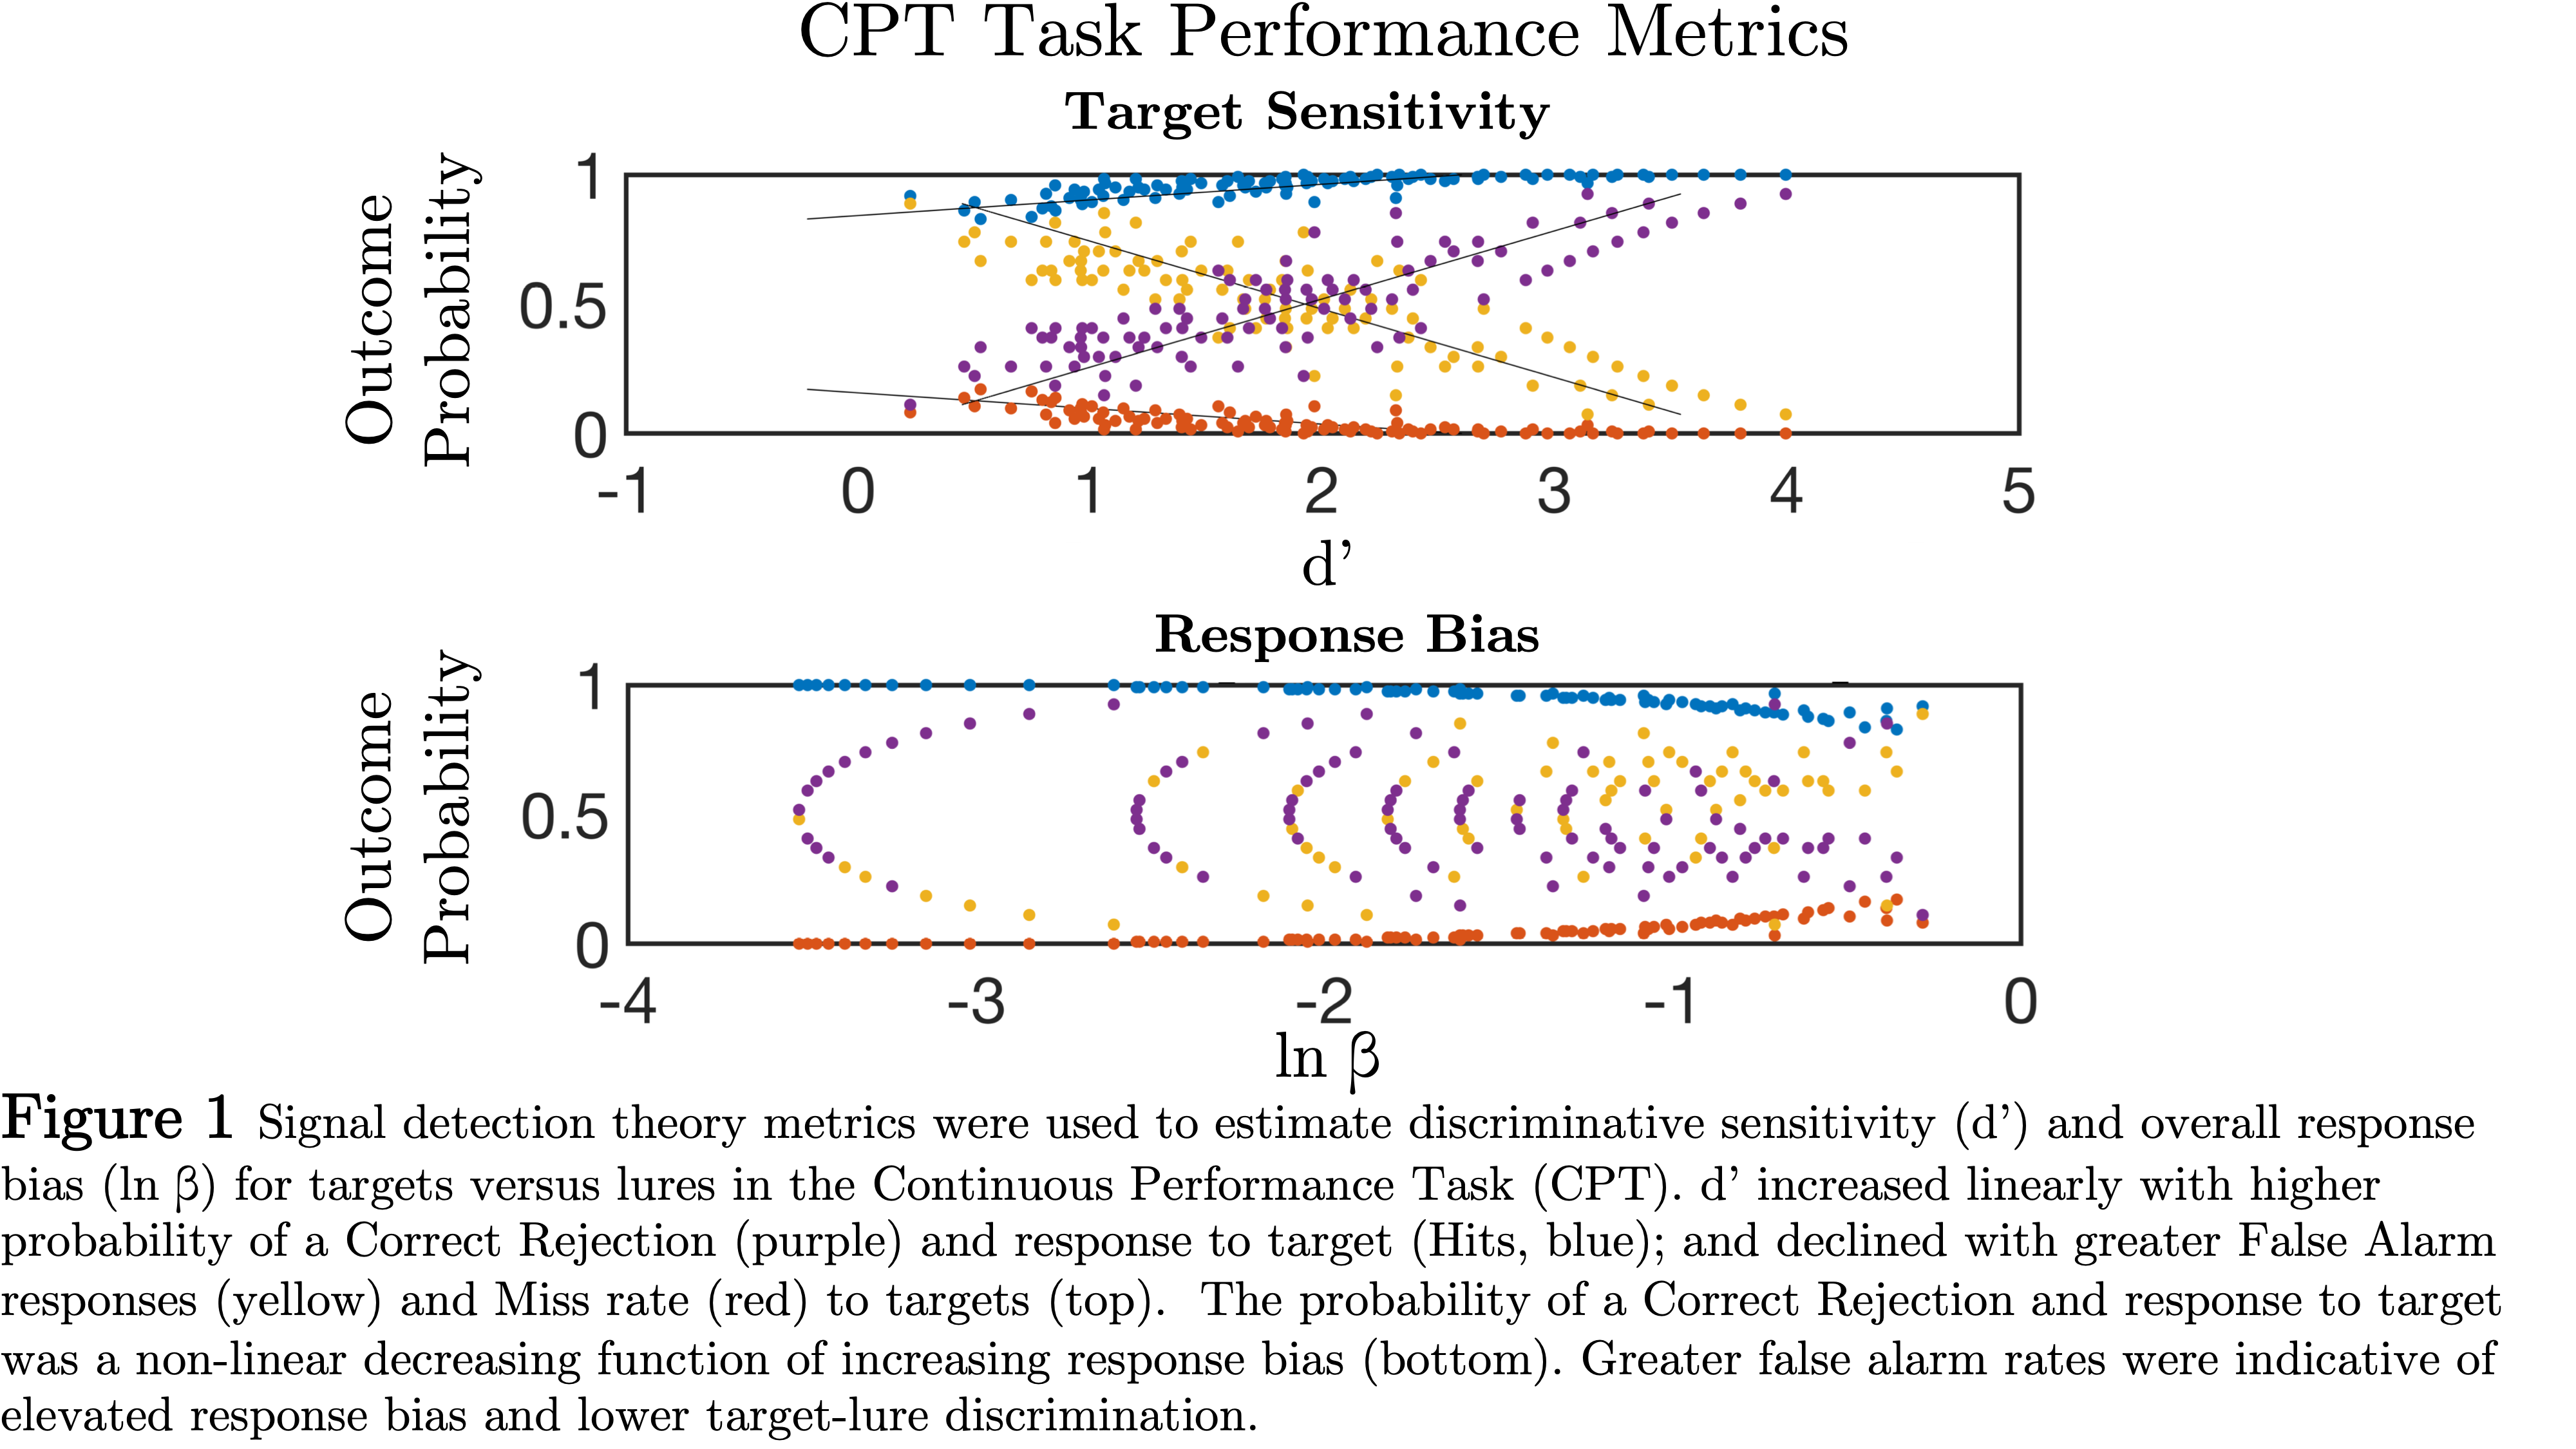
\includegraphics[width=\textwidth,height=\textheight,keepaspectratio]{Fig-1}
\caption{\label{fig:1}}
\end{figure}
%
\begin{figure}[h!]
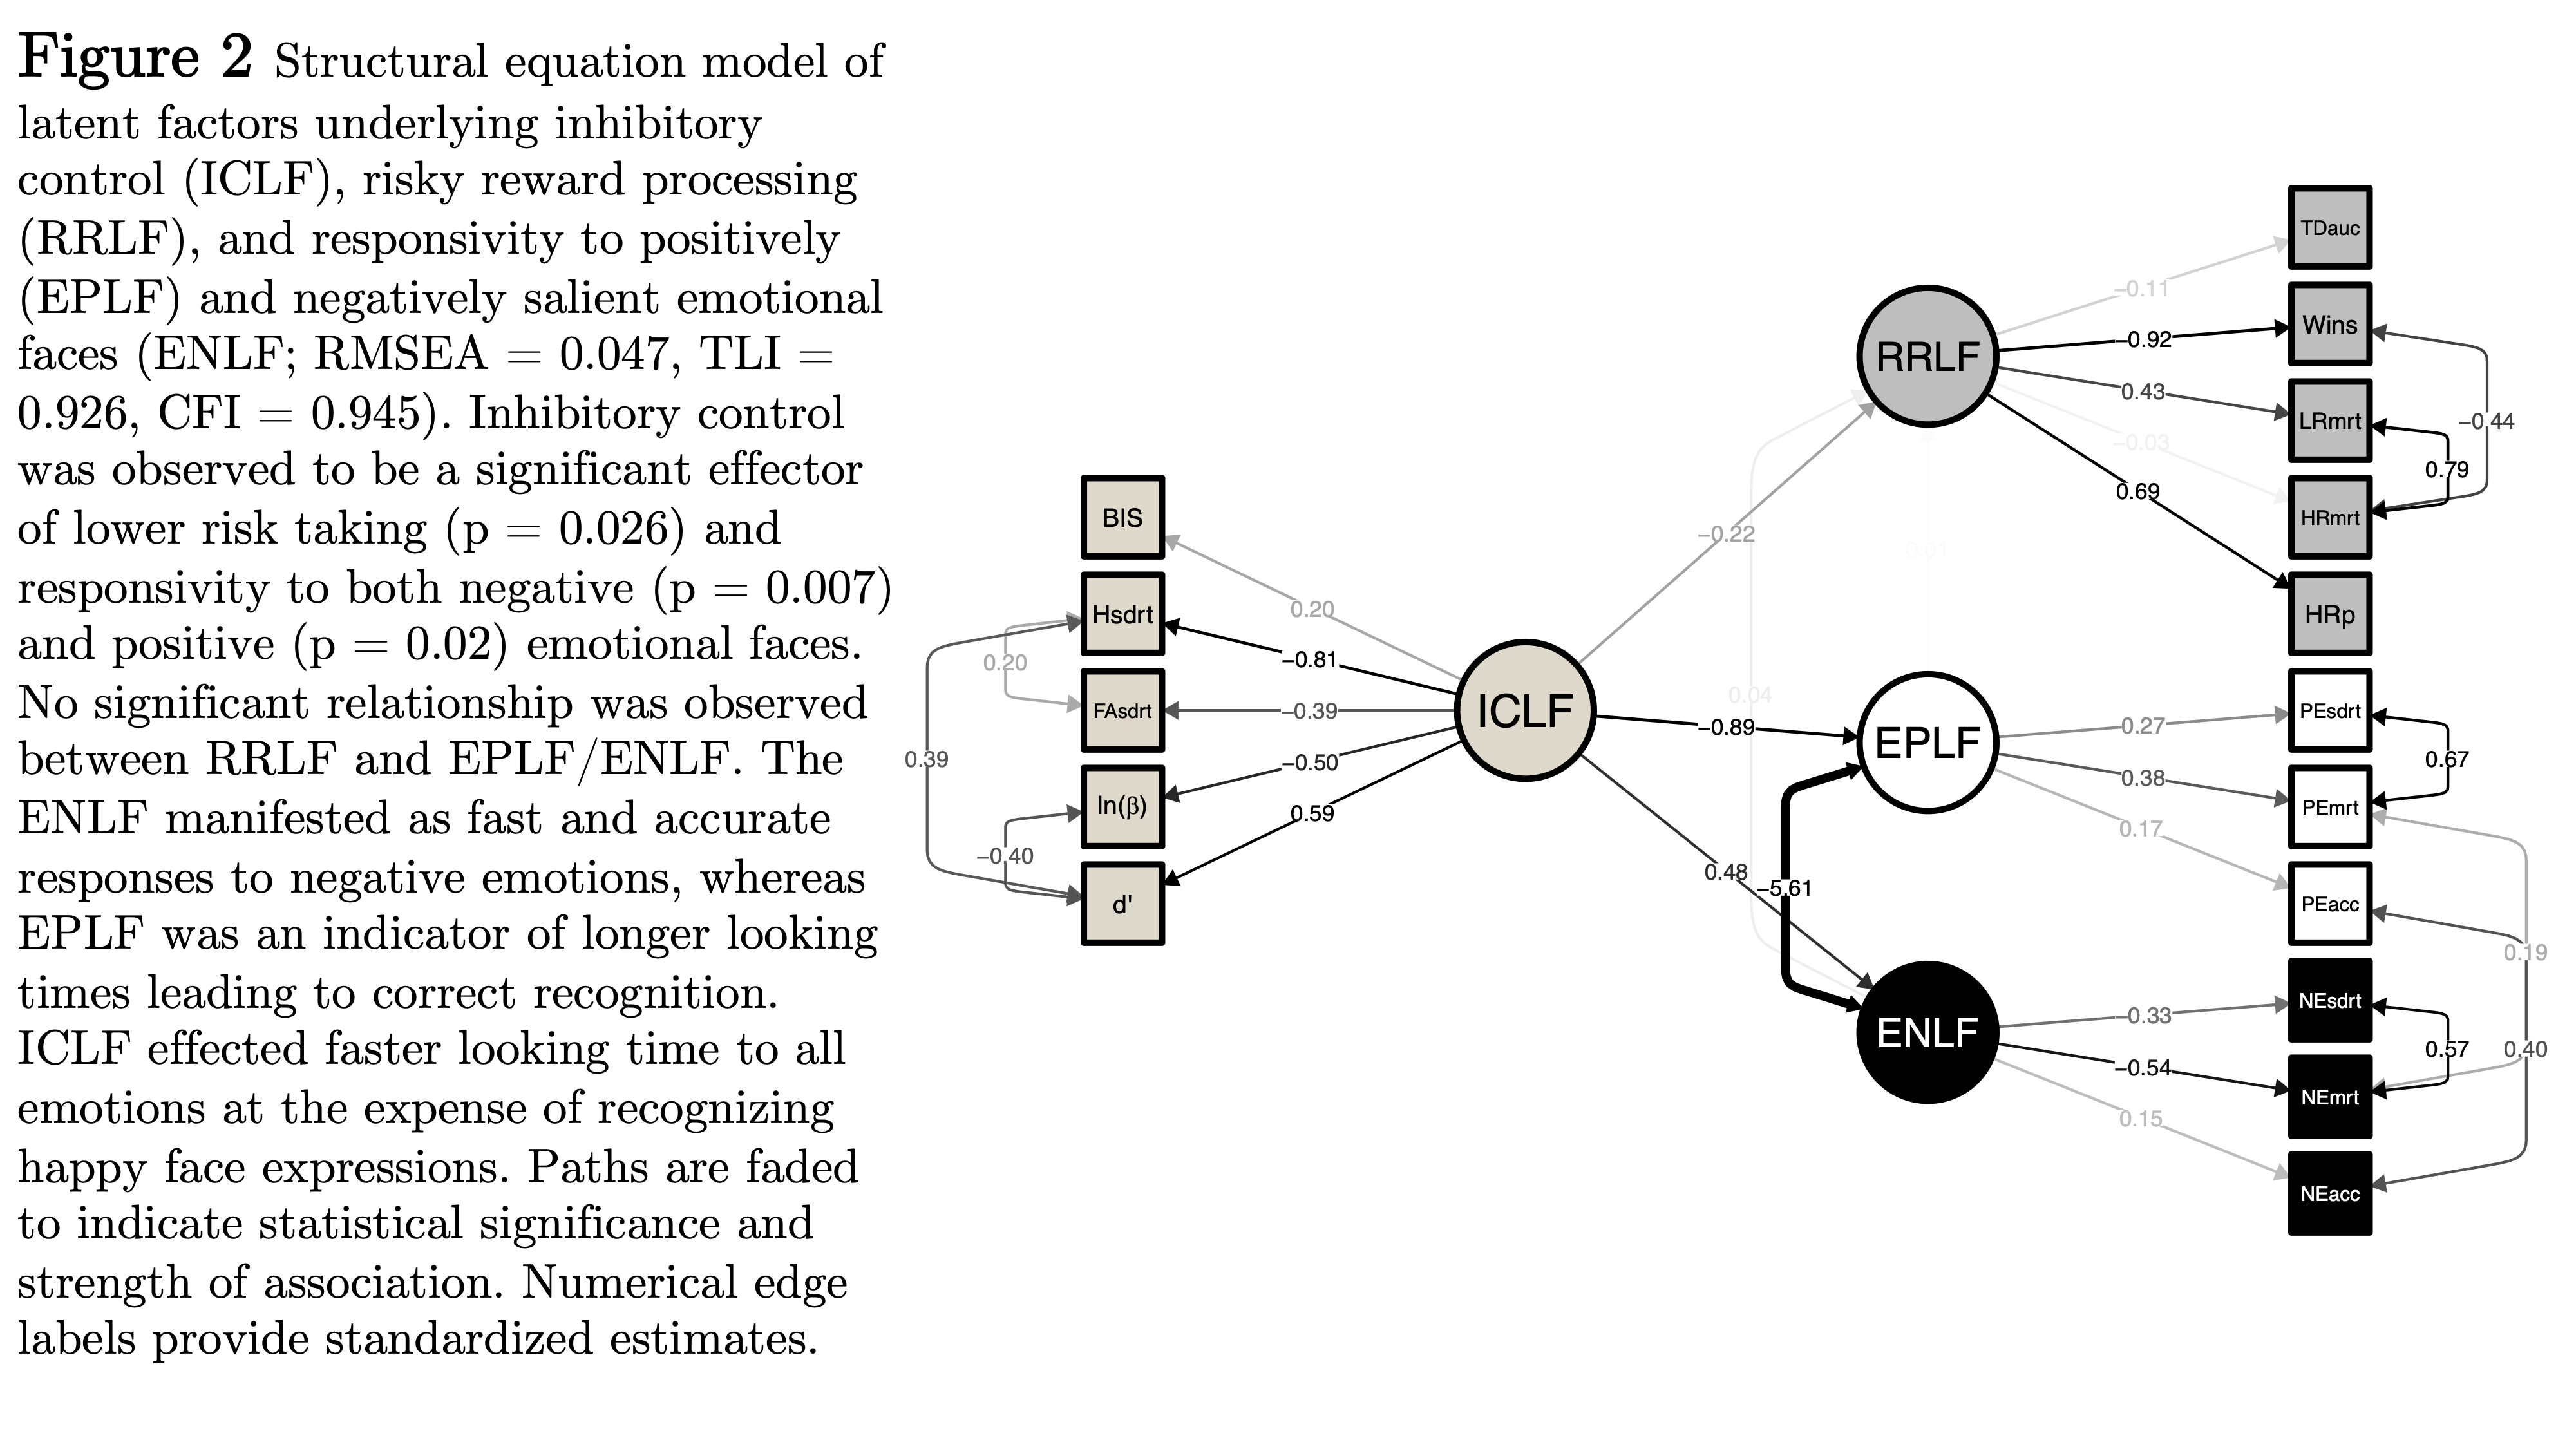
\includegraphics[width=\textwidth,height=\textheight,keepaspectratio]{Fig-2}
\caption{\label{fig:2}}
\end{figure}
%
\begin{figure}[h!]
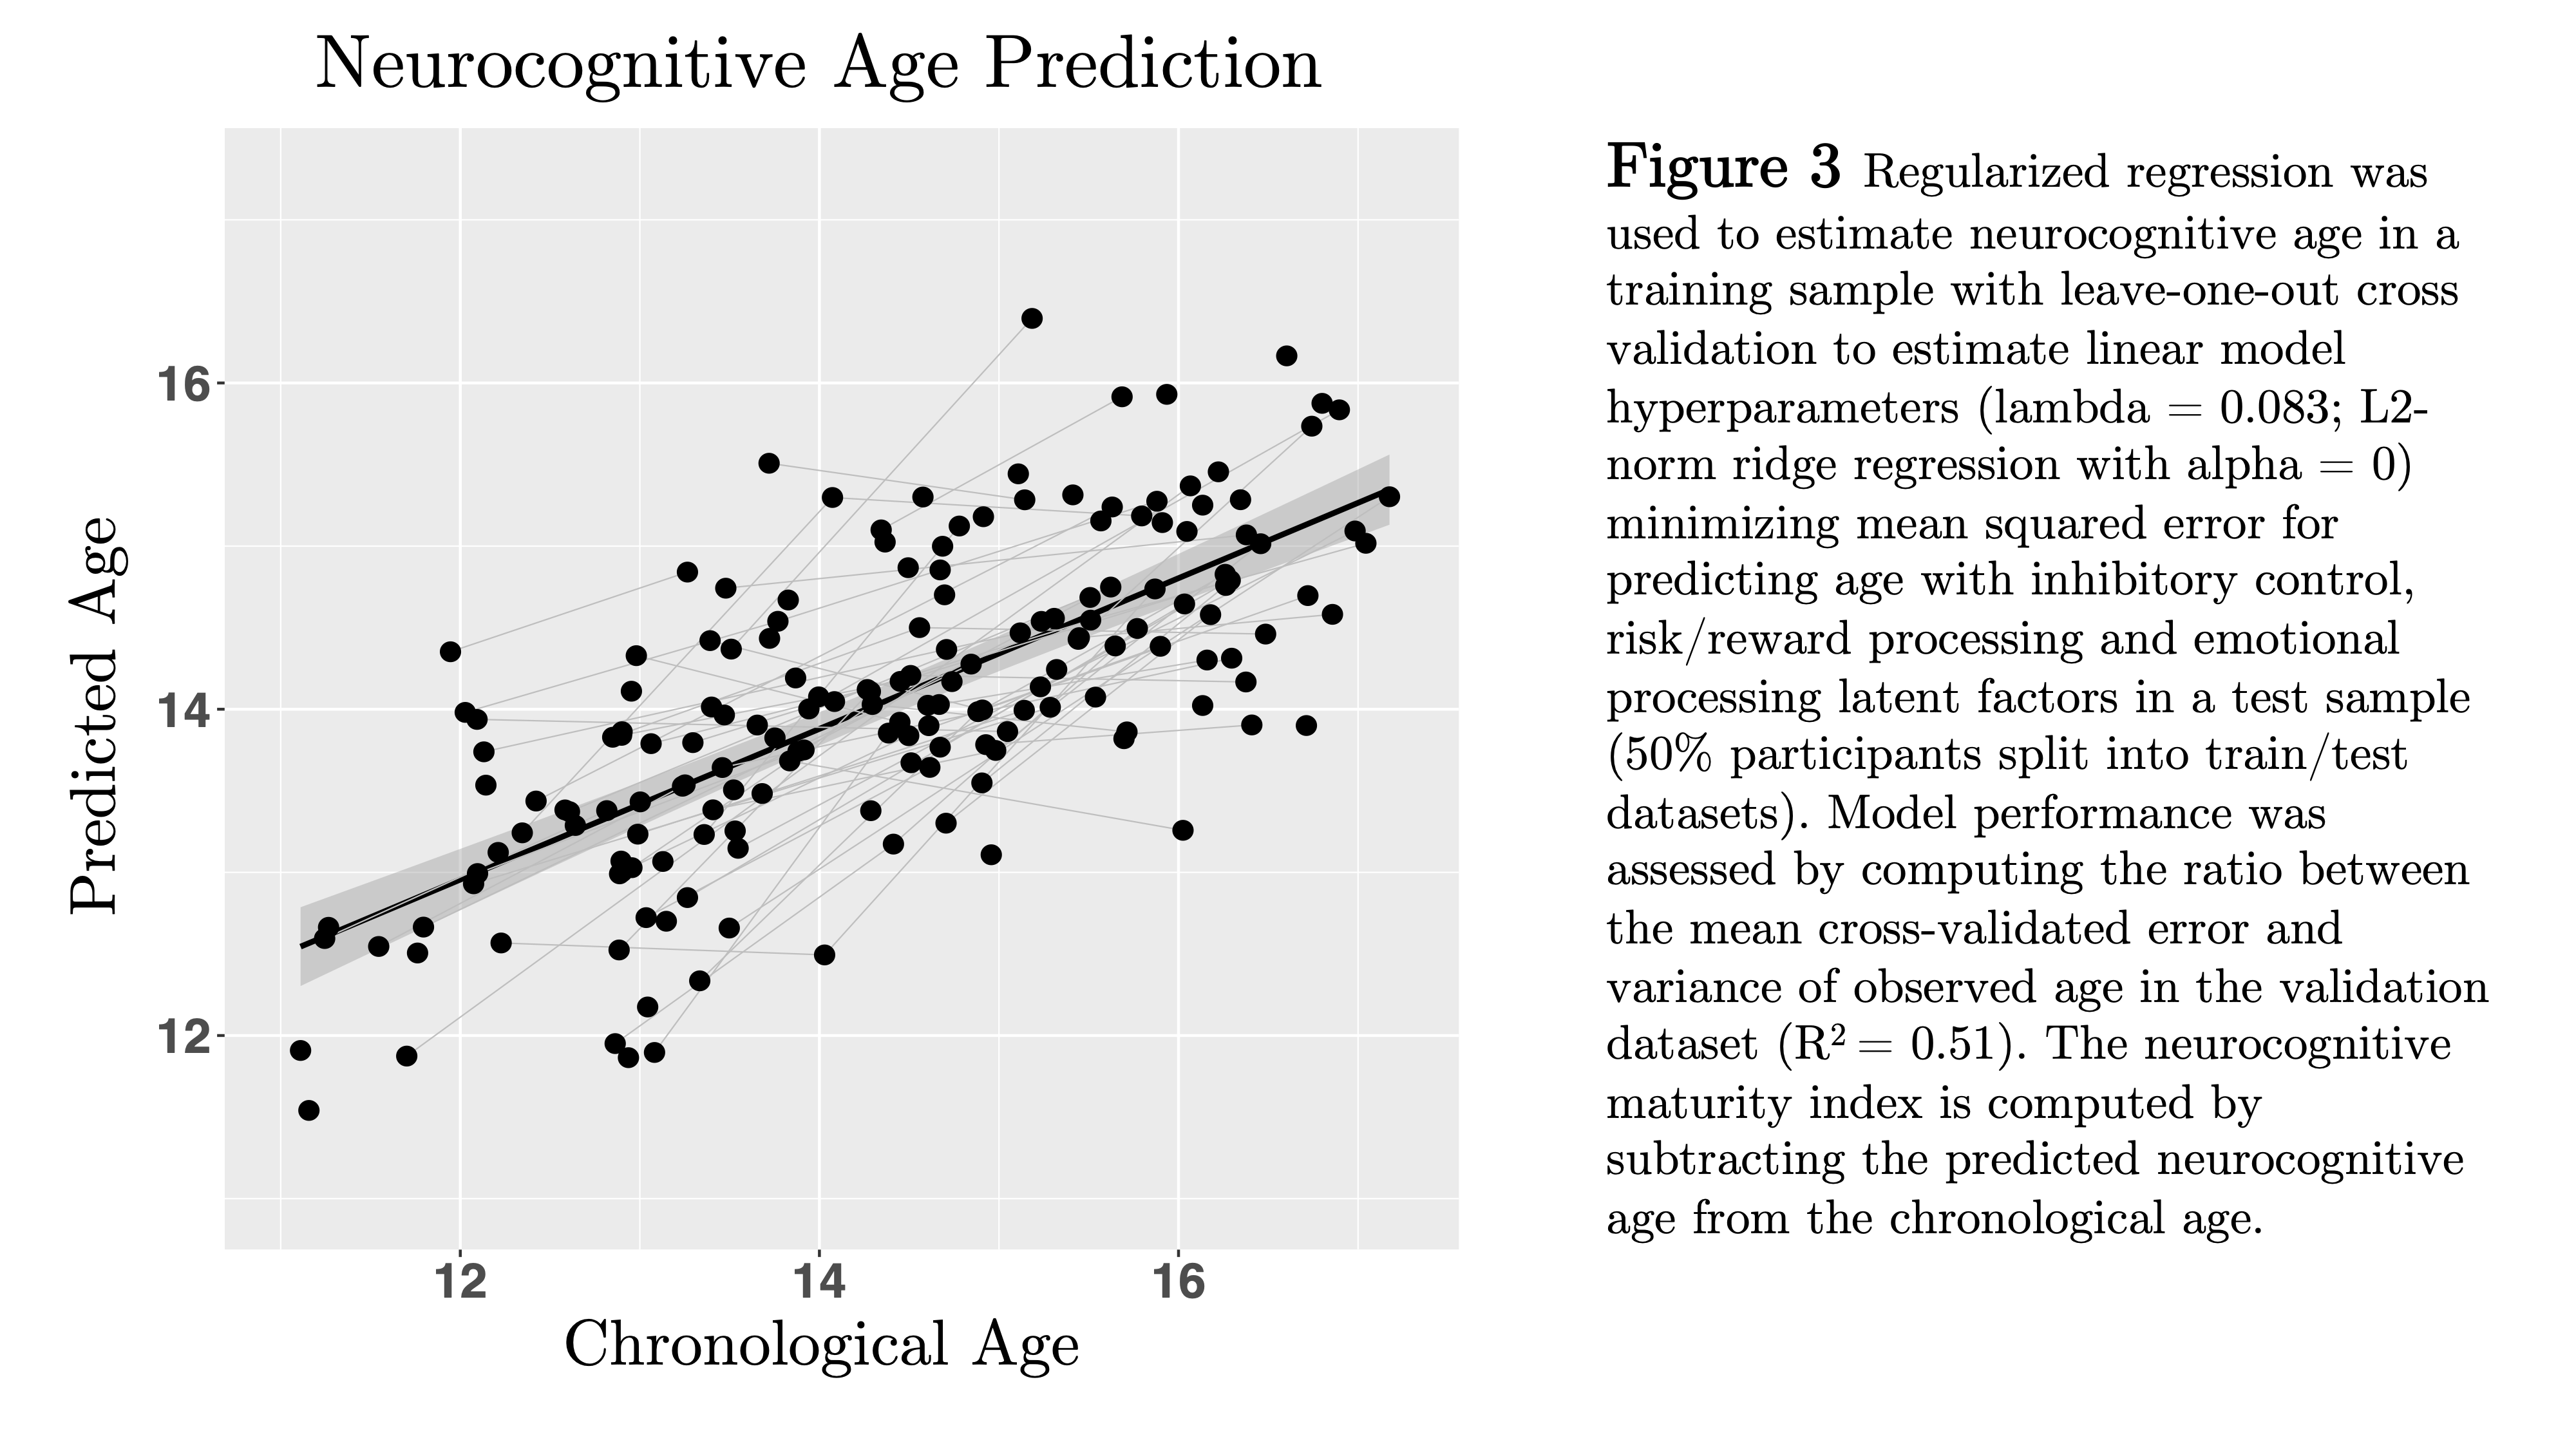
\includegraphics[width=\textwidth,height=\textheight,keepaspectratio]{Fig-3}
\caption{\label{fig:3}}
\end{figure}
%
\begin{figure}[h!]
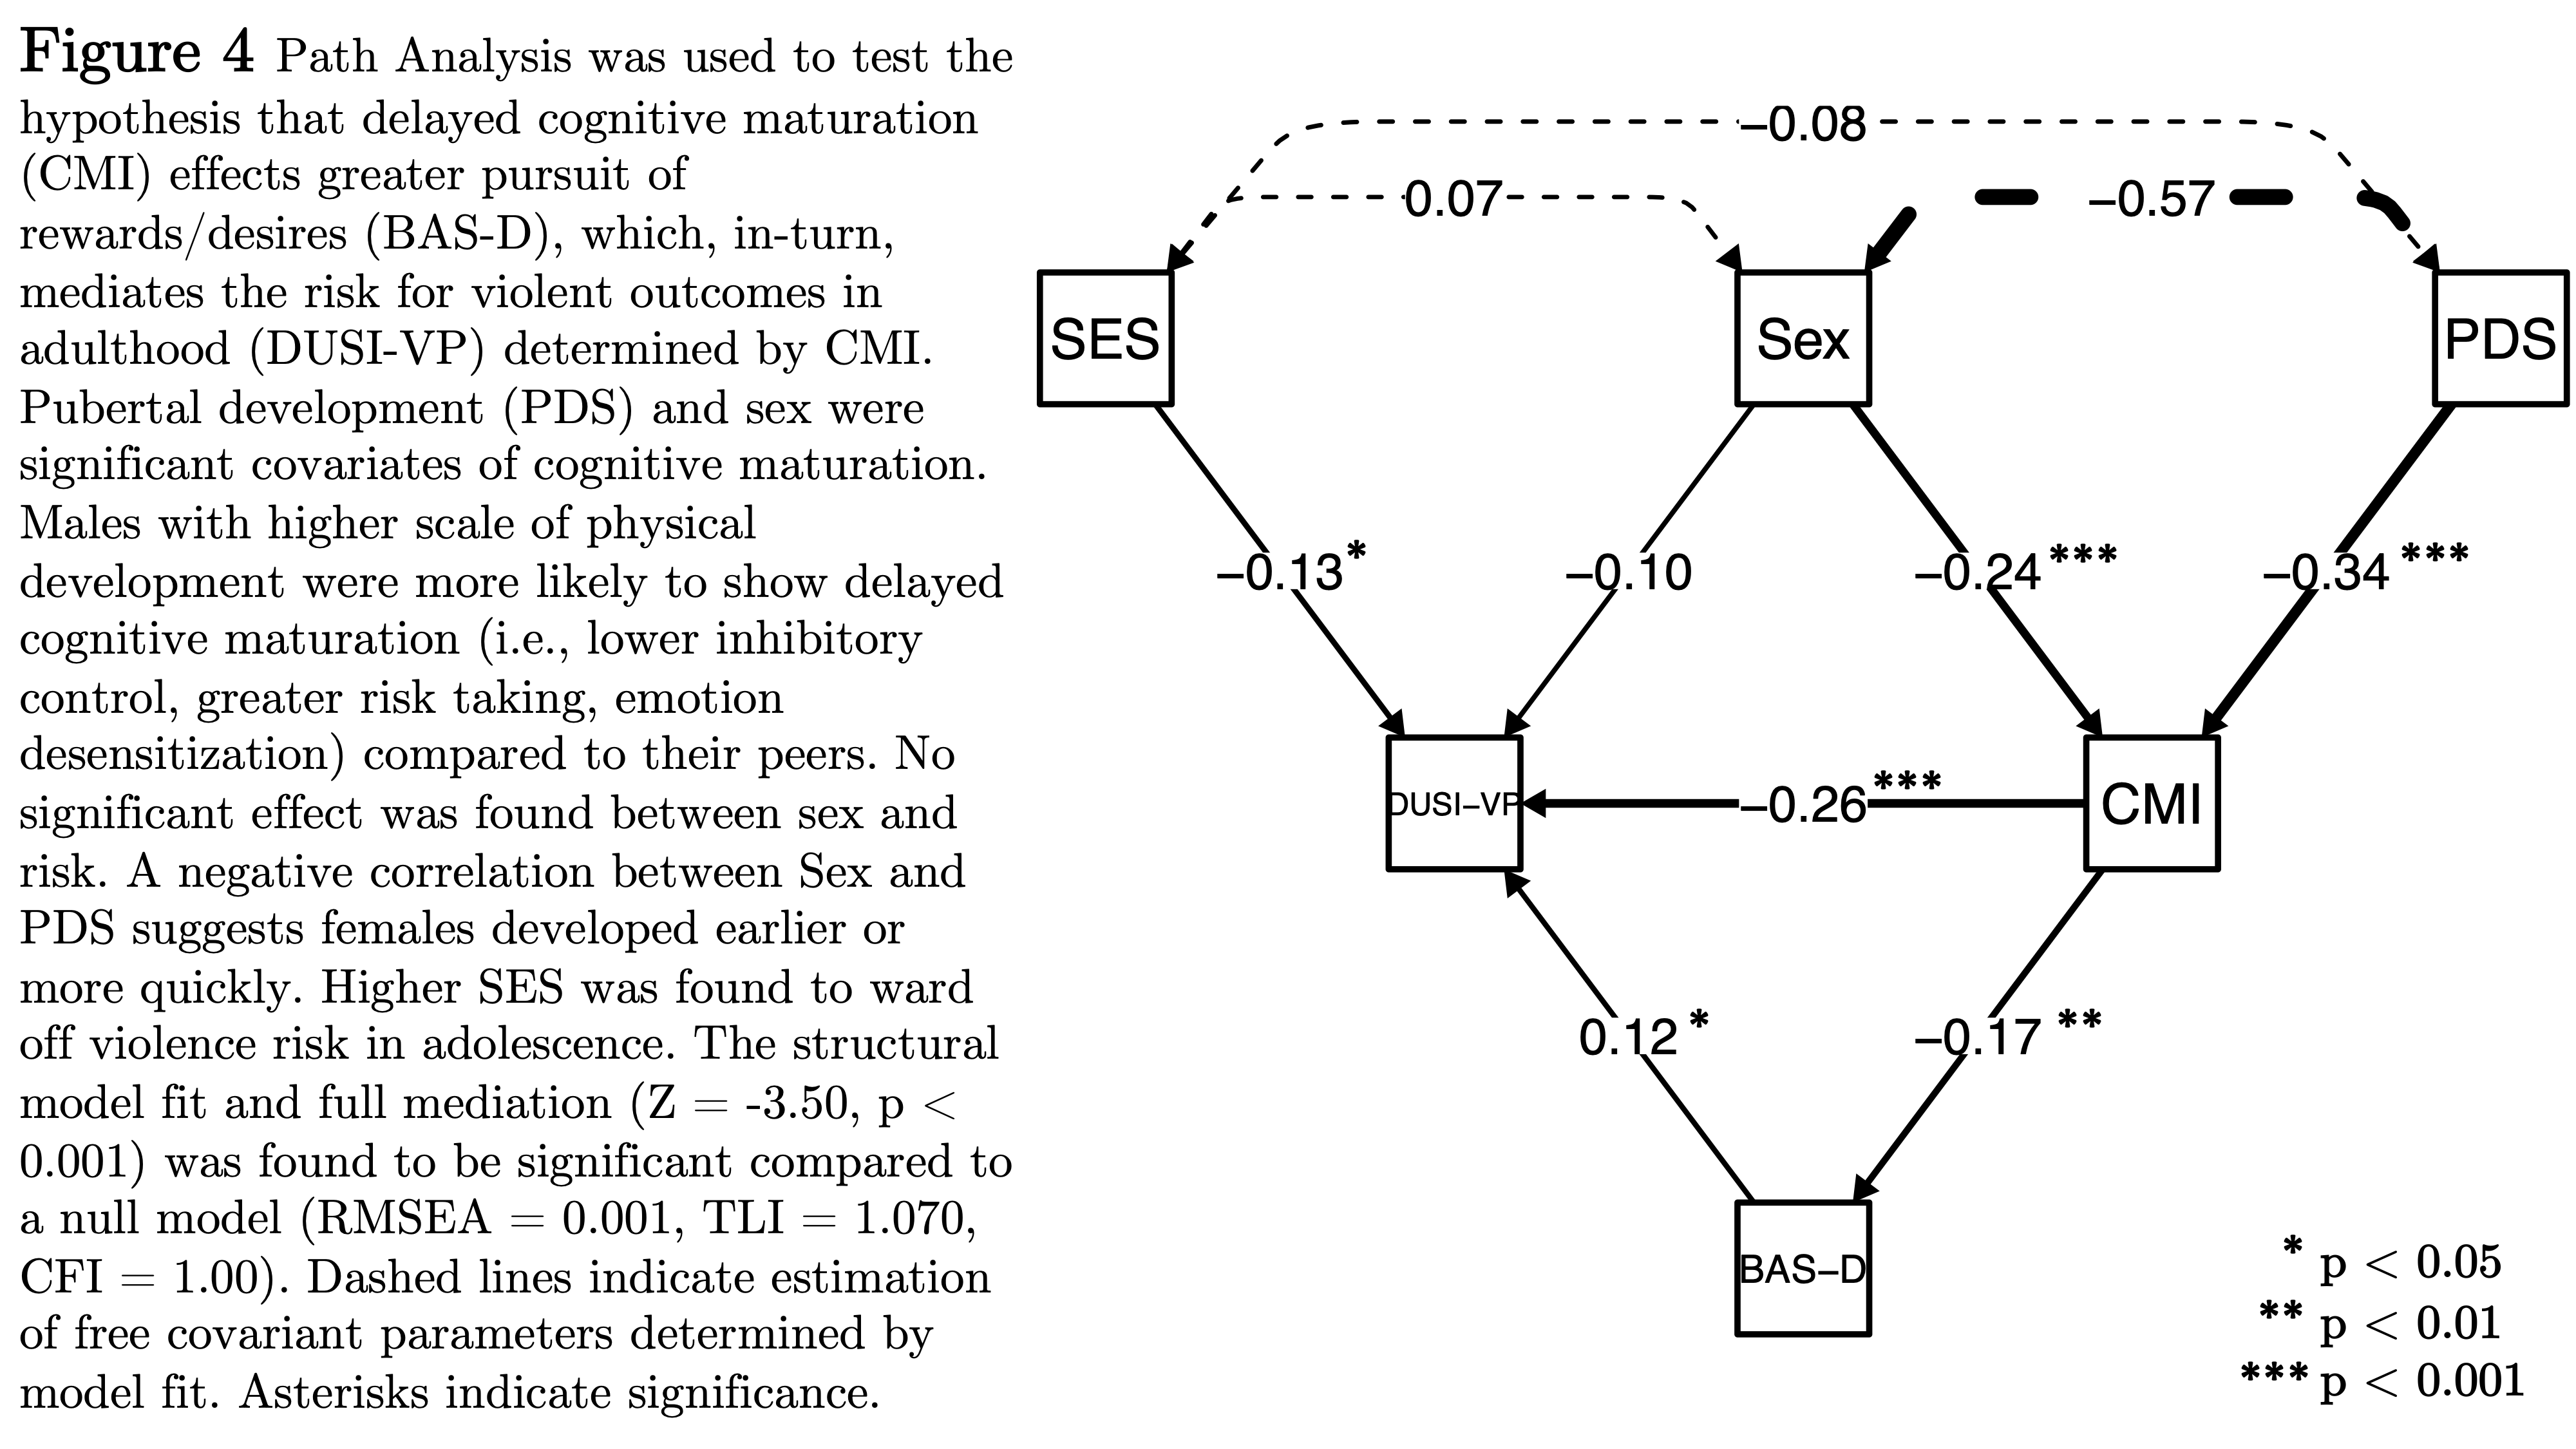
\includegraphics[width=\textwidth,height=\textheight,keepaspectratio]{Fig-4}
\caption{\label{fig:4}}
\end{figure}


\end{document}
